\documentclass{beamer}
\def\Put(#1,#2)#3{\leavevmode\makebox(0,0){\put(#1,#2){#3}}}
\usepackage{tabularx, booktabs}
\usetheme{Frankfurt}
\usepackage{caption}
\usepackage{color}
\usepackage{epsfig}
\usepackage{epstopdf}
\usepackage{pdfpages}
\usepackage{subfigure}


\captionsetup[table]{labelformat = empty}
\setbeamertemplate{navigation symbols}{} % Suppress the navigation symbols that normally appear on the bottom of Beamer slides

% Redefine the footer to three-panel split with Author | Title | Slide number instead of Warsaw default
\makeatletter
\setbeamertemplate{footline}
{
  \leavevmode%
  \hbox{%
  \begin{beamercolorbox}[wd=.25\paperwidth,ht=2.25ex,dp=1ex,center]{author in head/foot}%
    \usebeamerfont{author in head/foot}\insertshortauthor%~~\beamer@ifempty{\insertshortinstitute}{}{(\insertshortinstitute)}
  \end{beamercolorbox}%
  \begin{beamercolorbox}[wd=.5\paperwidth,ht=2.25ex,dp=1ex,center]{title in head/foot}%
    \usebeamerfont{title in head/foot}\insertshorttitle
  \end{beamercolorbox}%
  \begin{beamercolorbox}[wd=.25\paperwidth,ht=2.25ex,dp=1ex,right]{date in head/foot}%
   % \usebeamerfont{date in head/foot}\insertshortdate{}\hspace*{2em}
    \insertframenumber{} / \inserttotalframenumber\hspace*{2ex} 
  \end{beamercolorbox}}%
  \vskip0pt%
}
\makeatother


\title{Team 40: Mortality Prediction in ICU \ \newline CSE 6250 Final Project}
\author{Vincent La\footnote{vincent.la@gatech.edu}, Avi Ananthakrishnan\footnote{avinash.ananthakrishnan@gatech.edu}}
\institute{Georgia Tech}
\date{\today}

\begin{document}

\maketitle

\begin{frame}
\label{Presentation Outline 1}
\frametitle{Presentation Outline}
\begin{enumerate}
\item[1.] \textbf{Research Question}
\newline
\item[2.] Brief Review of Existing Literature and Background
\newline
\item[3.] Data
\newline
\item[4.] Empirical Design
\newline
\item[5.] Results
\newline
\item[6.] Future Considerations
\end{enumerate}
\end{frame}

\begin{frame}
\label{Research Question}
\frametitle{Research Question}
\begin{itemize}
	\item Overall: Mortality Prediction in the ICU
	\newline
	\item Specific: What is the probability that a patient in the ICU will become deceased using static and demographic features, medical diagnoses, and topics from clinical notes?
\end{itemize}
\end{frame}

\begin{frame} 
\frametitle{Research Question}
\begin{itemize}
	\item Why do we care?
	\newline
		\begin{itemize}
			\item There is a plethora of literature on predicting mortality rates.
			\item Quick feedback loops can affect clinical decision making
			\newline
		\end{itemize}
	\item Can unstructured data be helpful?
	\newline
		\begin{itemize}
			\item Lots of potential meaningful information within medical charts and notes.
			\item Perform Topic Modeling (LDA) on the clinical notes to extract meaningful features
		\end{itemize}
\end{itemize}
\end{frame}

\begin{frame}
\label{Presentation Outline 2}
\frametitle{Presentation Outline}
\begin{enumerate}
\item[1.] Research Question
\newline
\item[2.] \textbf{Brief Review of Existing Literature and Background}
\newline
\item[3.] Data
\newline
\item[4.] Empirical Design
\newline
\item[5.] Results
\newline
\item[6.] Future Considerations
\end{enumerate}
\end{frame}

\begin{frame}
\label{Literature Review}
\frametitle{Review of Existing Literature}
Ghassemi (2014)
\begin{itemize}
\item Does a similar approach in predicting mortality using notes from ICU
\newline
\end{itemize}

Other Studies
\begin{itemize}
\item Desalvo (2005): Provides an interesting "baseline" model performance by predicting mortality using a question to the patient about their health

\item Siontis (2011): Overall Survey Study for mortality prediction
\end{itemize}
\end{frame}

\begin{frame}
\label{Presentation Outline 3}
\frametitle{Presentation Outline}
\begin{enumerate}
\item[1.] Research Question
\newline
\item[2.] Brief Review of Existing Literature and Background
\newline
\item[3.] \textbf{Data}
\newline
\item[4.] Empirical Design
\newline
\item[5.] Results
\newline
\item[6.] Future Considerations
\end{enumerate}
\end{frame}

\begin{frame}
\label{Data}
\frametitle{Data}
MIMIC III (Medical Information Mart for Intensive Care)
\begin{itemize}
\item Freely (deanonymized) available critical care database developed by MIT Lab for Computational Physiology
\item Contains about 40,000 Patients; 60,000 admissions, and 6,000 mortality events from Beth Israel Deaconess Medical Center between 2001 and 2012
\item Includes both structured and unstructured data (e.g. static and demographic features); unstructured data includes vitals, clinical notes)
\end{itemize}
\end{frame}

\begin{frame}
\label{Data: Descriptive Statistics}
\frametitle{Data: Descriptive Statistics}
Mortality Rate: About 12\%

\begin{figure}[H]
\centering
\caption{Admissions Deaths}
\label{AdmissionsDeaths}
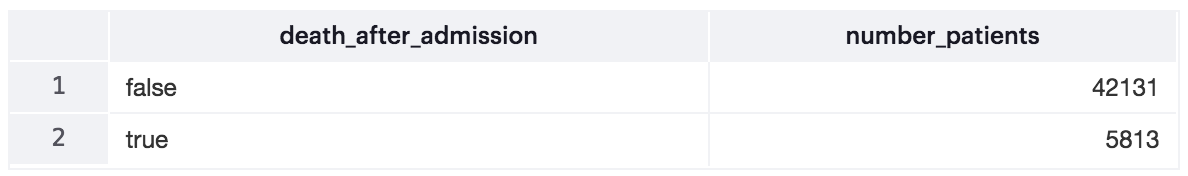
\includegraphics[page = {1}, scale = 0.4]{./images/admissions-deaths.png}
\end{figure}
\end{frame}

\begin{frame}
\frametitle{Data: Descriptive Statistics}
Most patients were admitted once to the hospital, a fraction were readmitted, and there is a right tail of patients who were admitted many times.

\begin{figure}[H]
\centering
\caption{Admissions Distribution}
\label{AdmissionsDistribution}
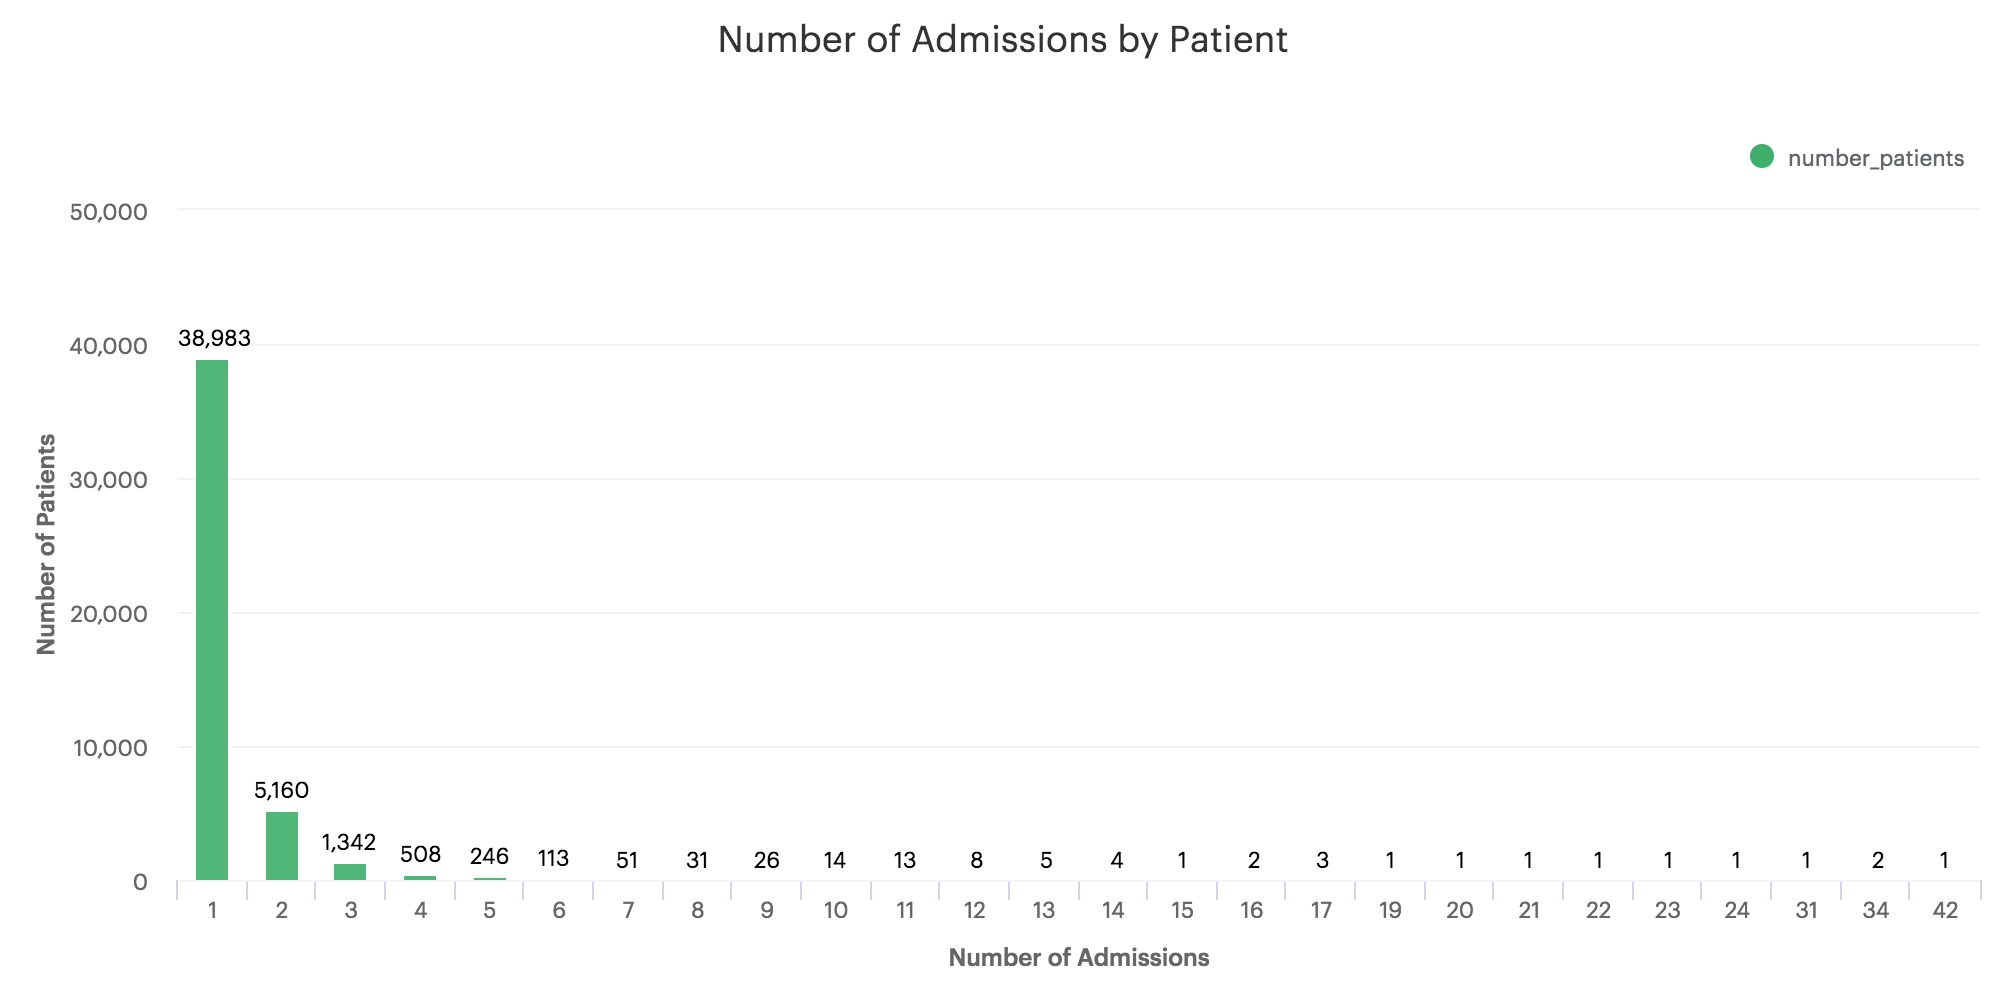
\includegraphics[page = {1}, scale = 0.2]{./images/admissions-distribution.png}
\end{figure}
\end{frame}

\begin{frame}
\frametitle{Data: Descriptive Statistics}
On average, patients were admitted for about 10 days, with the median closer to 6.5, suggesting large right skew.

\begin{figure}[H]
\centering
\caption{Admissions Lengths}
\label{AdmissionsLengths}
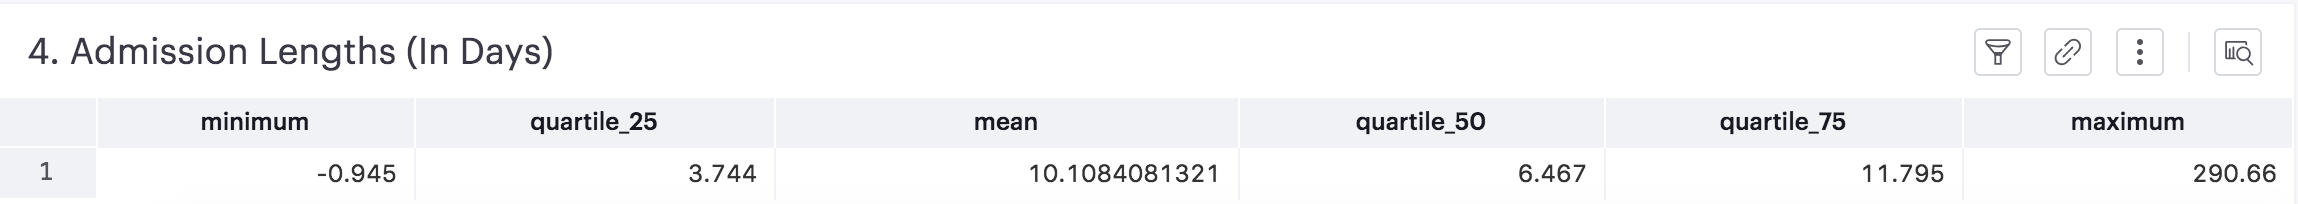
\includegraphics[page = {1}, scale = 0.2]{./images/admissions-lengths.png}
\end{figure}
\end{frame}

\begin{frame}
\frametitle{Data: Descriptive Statistics}
The modal patient is a Medicare patient, which makes sense since Medicare patients reflect higher risk and more likely to be in ICU setting.

\begin{figure}[H]
\centering
\caption{Admissions Insurance}
\label{AdmissionsInsurance}
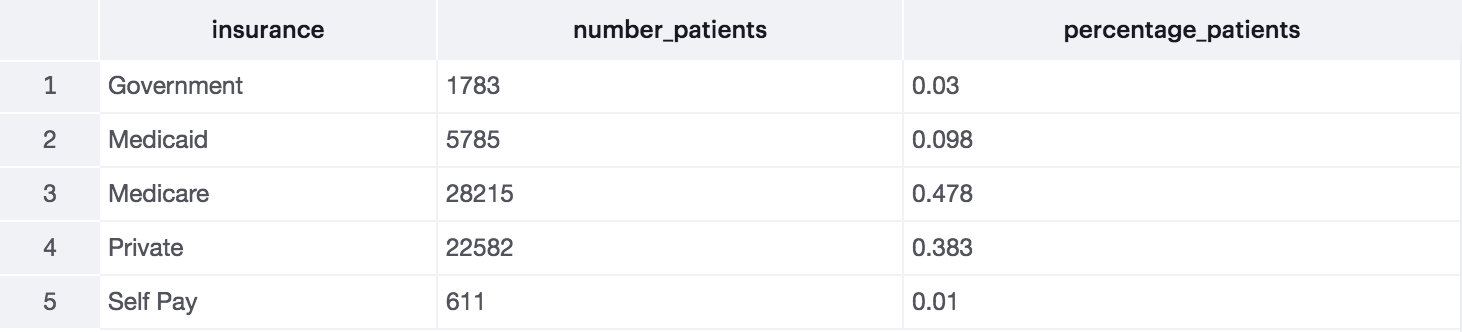
\includegraphics[page = {1}, scale = 0.4]{./images/admissions-insurance-summary.png}
\end{figure}
\end{frame}

\begin{frame}
\frametitle{Data: ETL and Tech Stack}
\label{ETL}
The tech stack that we use is:

\begin{itemize}
\item Python runtime
\item Hive + Hadoop
\item HBase data store
\item Run local to machine, did not use a hosted service like AWS EMR
\item Configuration of hive + Hadoop was tuned to available machine

  \begin{itemize}
    \item Local used default settings
    \item Full run of pipeline had increased parallelism to utilize resources quicker
  \end{itemize}
\end{itemize}
\end{frame}

\begin{frame}
\frametitle{Data: ETL and Tech Stack}
\label{ETL2}
\begin{itemize}
\item Pipeline was modeled as a set of scripts run
\item Starts with ETL of CSV files into HBase
\item Extracts features into HBase tables via HiveQL
\item HBase tables are transformed to Pandas data frames via HiveQL
\item ML models are run in Scikit-learn
\item Final model is exported as pickled Scikit-learn object
\end{itemize}
\end{frame}

\begin{frame}
\label{Presentation Outline 4}
\frametitle{Presentation Outline}
\begin{enumerate}
\item[1.] Research Question
\newline
\item[2.] Brief Review of Existing Literature and Background
\newline
\item[3.] Data
\newline
\item[4.] \textbf{Empirical Design}
\newline
\item[5.] Results
\newline
\item[6.] Future Considerations
\end{enumerate}
\end{frame}

\begin{frame}
\label{Empirical Design}
\frametitle{Feature Selection}

\begin{table}[H]
\tiny
\newcolumntype{C}{>{\centering\arraybackslash}X}% centering
\caption{Features}
\label{Features}
\centering
\begin{tabularx}{\textwidth}{l C C}\hline
 & (1) & (2) \\\
Categories & Features & Extracted \\ \hline
 &  &   \\
Demographic and Static Features & Age (at time of admission), Gender, Ethnicity, Admission Type, Insurance Type &  \\\
\\\
Clinical Diagnoses & Clinical Classification Software (CCS) Higher Level Categories & One Hot Encoded: 1 if Patient has diagnosis that maps to the CCS code during the admission, else 0 \\\
\\\
Clinical Notes & Topics using Latient Dirichlet Allocation (LDA) & Scores from Notes from the admission \\\
\end{tabularx}
\end{table}
\end{frame}

\begin{frame}
\label{Feature Selection: CCS}
\frametitle{Feature Selection: Diagnosis Data}

Diagnosis Data (ICD9)
\begin{itemize}
\item The International Classification of Diseases (ICD9) contains almost 65,000 total diagnosis codes.
\item With only 60,000 admissions, including all diagnosis codes will lead to very sparse data.
\end{itemize}

Clinical Classification Software (CCS) Codes

\begin{itemize}
\item To extract higher level and clinically meaningful classifications, we use the CCS ontologies produced by AHRQ via HCUP
\item CCS provides a many to one mapping of diagnosis codes to about 200 CCS codes which is helpful to reduce dimensionality and also is more clinically meaningful.
\end{itemize}
\end{frame}

\begin{frame}
\label{Feature Selection: Topic Modeling}
\frametitle{Feature Selection: Topic Modeling}

Latent Dirichlet Allocation (LDA) Topic Modeling

\begin{itemize}
\item Performed LDA on Note Events data to extract topics from notes recorded during an admission
\item Extracted a total of 10 topics.
\item For each document, we scored the probability that the topic was relevant to the document.
\item To construct the feature, we summed the scores for each patient-admission.
\end{itemize}
\end{frame}

\begin{frame}
\label{Feature Selection: Topic Modeling}
\frametitle{Feature Selection: Topic Modeling}

Examples of Topics extracted from LDA\footnote{We would like to thank Dr. Kumar Dharmarajan, a geriatrician, who helped provide some clinical context on the top few topics that LDA abstracted.}

\begin{table}[H]
\footnotesize
\newcolumntype{C}{>{\centering\arraybackslash}X}% centering
\caption{Examples of Topics Returned by LDA}
\label{LDA}
\centering
\begin{tabularx}{\textwidth}{l C C}\hline
 & (1) \\\
Topic Number & Top Words \\ \hline
 &    \\\
0 & contrast, mass, head, imag, brain  \\\
1 & effus, pleural, lung, chang, portabl \\\
2 & spine, arteri, carotid, imag, cervic
\end{tabularx}
\end{table}
\end{frame}

\begin{frame}
\label{Model}
\frametitle{Model}

Random Forest Classifier

\begin{itemize}
\item We choose a Random Forest classifier as our main model to predict mortality
\item A non-parametric model like Random Forest can detect non-linearities and interactions that are likely present within the data but we don't know a priori.
\item 70\% Train vs. 30\% Test Split
\item Metrics: AUROC, and Precision-Recall
\end{itemize}
\end{frame}

\begin{frame}
\label{Presentation Outline 6}
\frametitle{Presentation Outline}
\begin{enumerate}
\item[1.] Research Question
\newline
\item[2.] Brief Review of Existing Literature and Background
\newline
\item[3.] Data
\newline
\item[4.] Empirical Design
\newline
\item[5.] \textbf{Results}
\newline
\item[6.] Future Considerations
\end{enumerate}
\end{frame}

\begin{frame}
\label{Results: Overview}
\frametitle{Results: Overview}
The main outcome variable is whether mortality was recorded in the hospital event after the admission. We present results from three models:

\begin{itemize}
\item Baseline Model: Only uses Demographic and Static Features (e.g. age at admission, gender, insurance, race)
\item Baseline + Clinical Diagnosis: Includes all the features from the Baseline model but also uses diagnosis data (with higher level groupings produced by CCS)
\item Baseline + Clinical Diagnosis + Clinical Notes: Includes all the features from Baseline and Diagnosis data and also uses abstracted topics from Note Events using LDA.
\end{itemize}
\end{frame}

\begin{frame}
\frametitle{Results: Baseline Model}

Model Metrics: AUROC (70\%); AU(PR)C (18\%)

\begin{figure}[H]
\centering     %%% not \center
\subfigure[ROC]{\label{fig:a}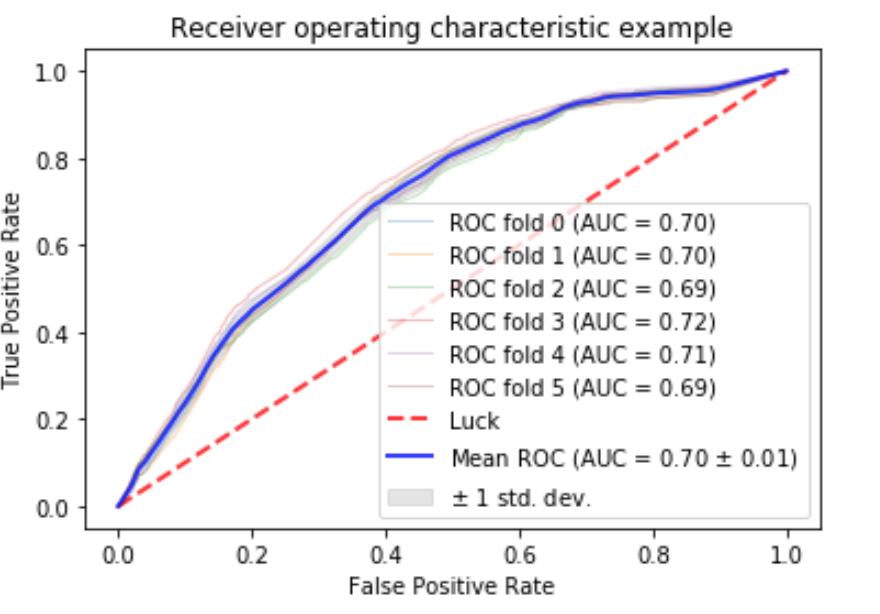
\includegraphics[width=35mm]{./images/modelperformance-baseline-roc}}
\subfigure[Precision Recall]{\label{fig:b}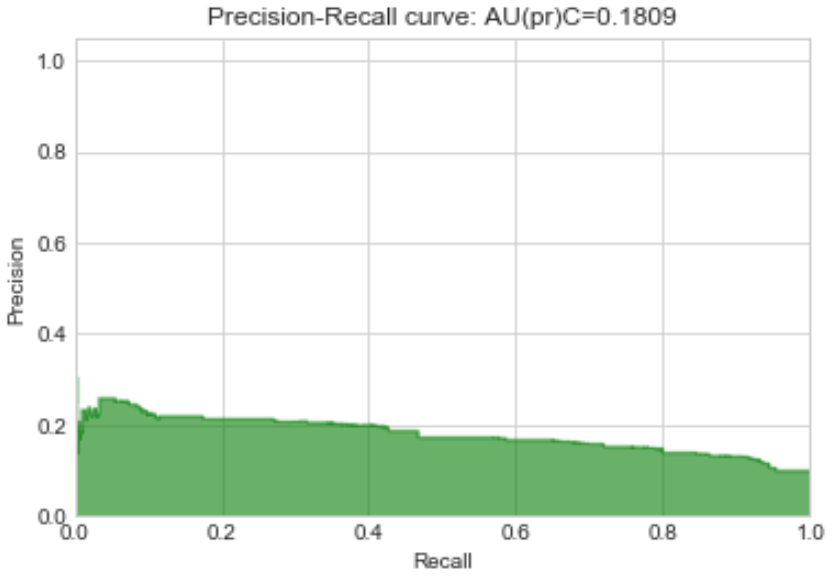
\includegraphics[width=35mm]{./images/modelperformance-baseline-pr}}
\caption{Baseline Model Performance}
\label{BaselineModelPerformance}
\end{figure}
\end{frame}

\begin{frame}
\frametitle{Results: Baseline + Clinical Diagnosis Model}

Model Metrics: AUROC (83\%); AU(PR)C (36\%)

\begin{figure}[H]
\centering     %%% not \center
\subfigure[ROC]{\label{fig:a}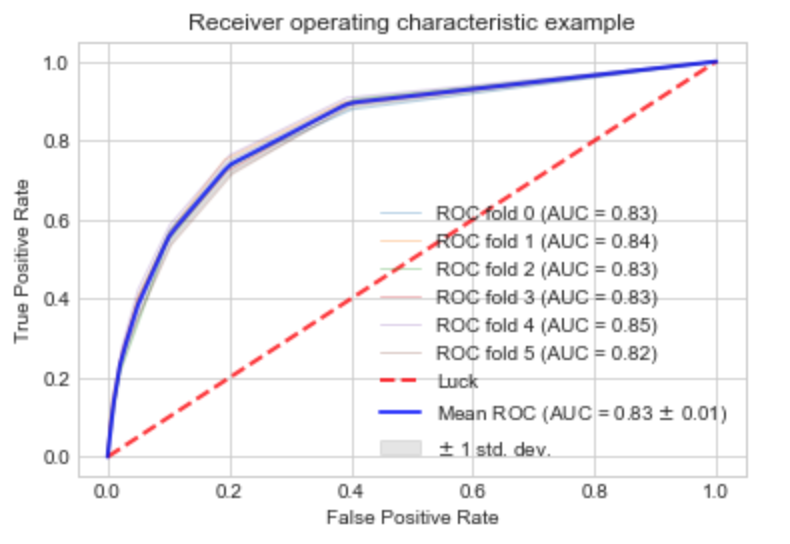
\includegraphics[width=35mm]{./images/modelperformance-improved-roc}}
\subfigure[Precision Recall]{\label{fig:b}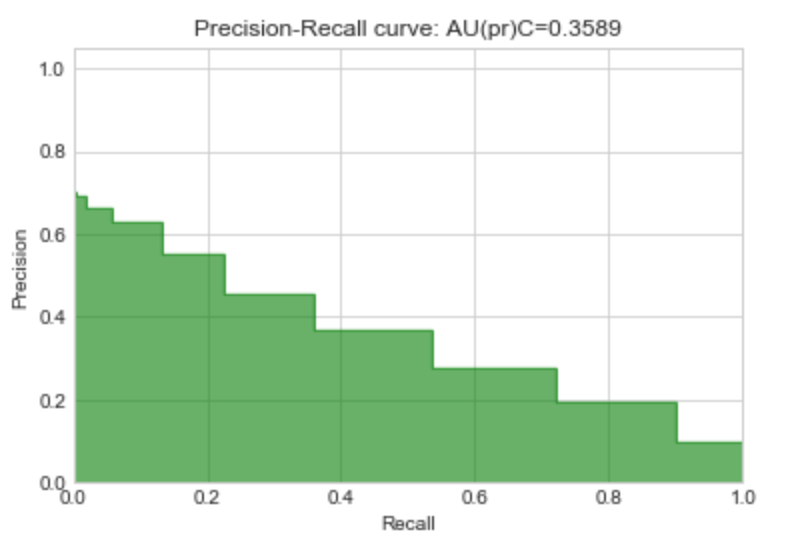
\includegraphics[width=35mm]{./images/modelperformance-improved-pr}}
\caption{Baseline + Clinical Diagnosis Model Performance}
\label{ImprovedModelPerformance}
\end{figure}
\end{frame}

\begin{frame}
\frametitle{Results: Baseline + Clinical Diagnosis + Clinical Notes Model}

Model Metrics: AUROC (83\%); AU(PR)C (42\%)

\begin{figure}[H]
\centering     %%% not \center
\subfigure[ROC]{\label{fig:a}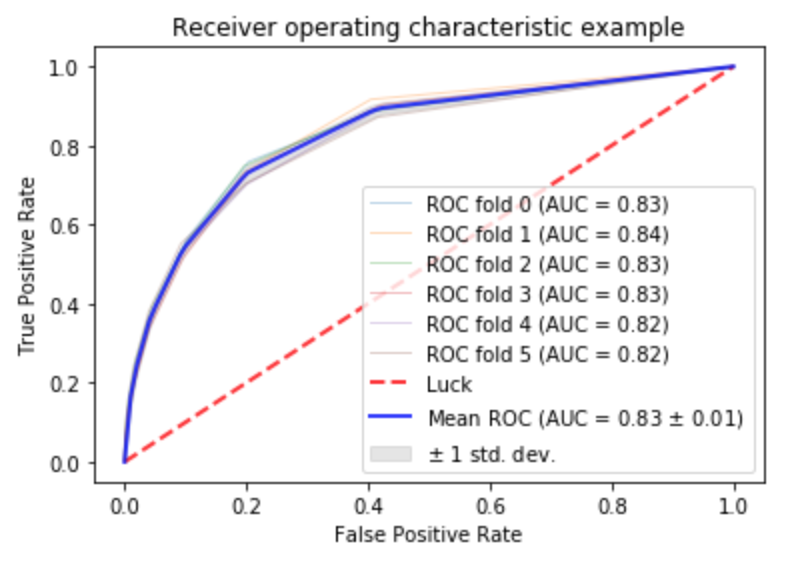
\includegraphics[width=35mm]{./images/modelperformance-best-roc}}
\subfigure[Precision Recall]{\label{fig:b}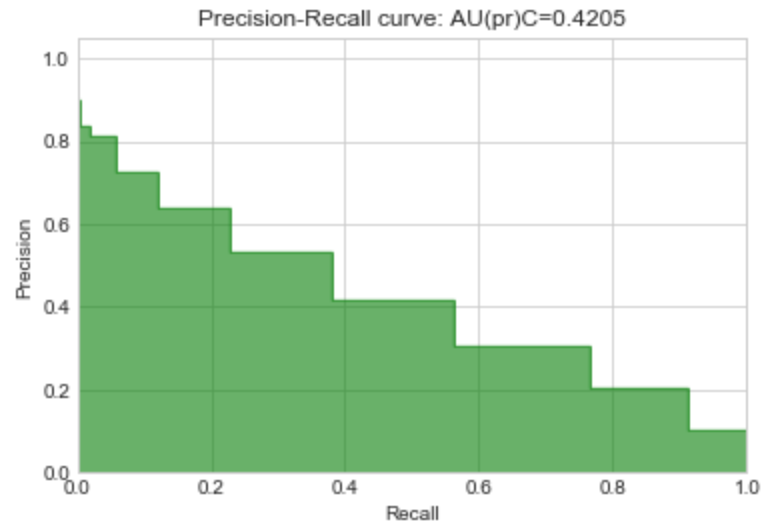
\includegraphics[width=35mm]{./images/modelperformance-best-pr}}
\caption{Baseline + Clinical Diagnosis + Clinical Notes Model Performance}
\label{BestModelPerformance}
\end{figure}
\end{frame}

\begin{frame}
\label{Presentation Outline 7}
\frametitle{Presentation Outline}
\begin{enumerate}
\item[1.] Research Question
\newline
\item[2.] Brief Review of Existing Literature and Background
\newline
\item[3.] Data
\newline
\item[4.] Empirical Design
\newline
\item[5.] Results
\newline
\item[6.] \textbf{Future Considerations}
\end{enumerate}
\end{frame}

\begin{frame}
\label{Conclusion}
\frametitle{Conclusion}
\begin{itemize}
\item[1] Even just using static and demographic features provides some predictive power
	\begin{itemize}
		\item Age at time of admission was an important feature, along with insurance type (which makes sense as this is a proxy for risk).
	\end{itemize}
\item[2] Model significantly improves with diagnosis data and clinical notes
	\begin{itemize}
		\item Using CCS Diagnosis codes significantly improved model performance 
		\item Using Clinical Notes improved Precision-Recall tradeoff which would be very useful in clinical setting
	\end{itemize}
\item[3] \textbf{Next step would be to talk with clinicians and improve interpretability of the model to make it actionable in a clinical setting!}
\end{itemize}
\end{frame}

\end{document}
